\title{Master Project - Real Time Rendering of skeletal structures - Motivations Goals and Plan}
\author{
        %\large
        \textsc{Olivier Rouiller - s090842}
        \mbox{}\\ %
        Department of Informatics and Mathematical Modelling\\
        Technical University of Denemark\\
        \mbox{}\\ %
}
\date{\today}
\documentclass[11pt]{article}
%\documentclass{acmconf}

\usepackage[paper=a4paper,dvips,top=1.5cm,left=1.5cm,right=1.5cm,
    foot=1cm,bottom=1.5cm]{geometry}

\usepackage{times}
%\usepackage{graphicx}
\usepackage[fleqn]{amsmath}
\usepackage{amsfonts}
\usepackage{amssymb}
\usepackage{amsthm}
\usepackage{amsopn}
\usepackage{xspace}
\usepackage{array}
\usepackage{epsfig}
\usepackage{cite}
\usepackage{pdfpages} 


\numberwithin{figure}{section}

\newcommand\CC{\Lang{\mbox{C++}}\xspace}
\newcommand\Lang[1]{\textsc{#1}}
\newcommand{\kw}[1]{\texttt{\textbf{#1}}}
\newcommand{\cd}[1]{\texttt{#1}}

\newcommand\Naturals{\ensuremath{\mathbb{N}}\xspace}
\newcommand\Integers{\ensuremath{\mathbb{Z}}\xspace}
\newcommand\Rationals{\ensuremath{\mathbb{Q}}\xspace}
\newcommand\Reals{\ensuremath{\mathbb{R}}\xspace}
\newcommand\Complex{\ensuremath{\mathbb{C}}\xspace}

\newcommand\norm[1]{\ensuremath{\lVert#1\rVert}}
\newcommand\abs[1]{\ensuremath{\lvert#1\rvert}}
\newcommand\ceil[1]{\ensuremath{\lceil#1\rceil}}
\newcommand\floor[1]{\ensuremath{\lfloor#1\rfloor}}
\newcommand\set[1]{\ensuremath{\{#1\}}}
\newcommand\angular[1]{\ensuremath{\langle#1\rangle}}

\newcommand\Norm[1]{\ensuremath{\left\lVert#1\right\rVert}}
\newcommand\Abs[1]{\ensuremath{\left\lvert#1\right\rvert}}
\newcommand\Ceil[1]{\ensuremath{\left\lceil#1\right\rceil}}
\newcommand\Floor[1]{\ensuremath{\left\lfloor#1\right\rfloor}}
\newcommand\Set[1]{\ensuremath{\left\{#1\right\}}}
\newcommand\Angular[1]{\ensuremath{\left\langle#1\right\rangle}}

\newcommand{\LOOM}{\ensuremath{\cal{LOOM}}\xspace}
\newcommand{\PolyTOIL}{\textbf{PolyTOIL}\xspace}

\newtheorem{theorem}{Theorem}[section]
\newtheorem{definition}[theorem]{Definition}
\newtheorem{lemma}[theorem]{Lemma}
\newtheorem{corollary}[theorem]{Corollary}
\newtheorem{fact}[theorem]{Fact}
\newtheorem{example}[theorem]{Example}

\newcommand\Cls[1]{\textsf{#1}}
\newcommand\Fig[1]{Figure~\ref{Figure:#1}}

\usepackage{labels} %
\usepackage{equation}
\usepackage{prog2tex}

\newenvironment{excerpt}{\begin{quote}\begin{minipage}\textwidth}{\end{minipage}\end{quote}}

\setcounter{topnumber}{0}
\setcounter{bottomnumber}{0}
\setcounter{totalnumber}{20}
\renewcommand{\textfraction}{0.01}

\begin{document}

\maketitle

\Section[simple]{Related Work}
\subsection{Skeletal modeling}
Surfaces defined by skeletal structures have been popular in Computer Graphics, applications in modelling are possible, mesh generation of organic structures such as trees, blood vessels have been done using skeletal structures. A skeletal structure can easily be generated with L-Systems.

In addition, modelling at a polygon level requires expert skills and is time consuming and a more compact representation of the models is useful to make the modelling easier and is interesting for procedural generation of content.

Bloomenthal \cite{Bloomenthal:1996:SDN:238973} used the idea that shapes are defined by their skeleton to model organic objects such as hands, leafs and trees. 
Implicit surfaces are suitable to define the geometry from a skeleton since their topology is robust.
The surface is represented as a convolution surface. Convolution surfaces offers large possibilities to create surfaces from discreet primitives. They have been studied thoroughly in Andrei Sherstyuk's thesis in \cite{Sherstyuk}.
This representation allows to define a smooth and topologically robust surface to primitive such as points, segments, curves, polygons or even meshes. These primitive are convoluted with distance functions such as Gaussians or other metaballs function and these fields are added or combined in different ways for blending. 

Wyvil et al. designed a data structure, the BlobTree to store these primitives and operations. \cite{Wyvill:98a}.

This approach have been studied for modelling of organic structures or characters.

\subsection{Skeletal meshing}
However generating meshes from implicit surfaces is hard. The most common algorithm is marching cubes \cite{Lorensen:1987:MCH:37402.37422} but it can fail to reconstruct small features if the resolution of the grid is too low and triangles are not aligned to the shapes's features. In addition, it generates a large number of polygons.
Some works have been done to use curvature information to reconstruct an implicit surface \cite{Araujo:2004:CDP:1025131.1026262} but the results are not good enough to be a viable alternative to marching cubes (more?).

Other approaches have been studied to generate meshes from skeletal structure, a class of algorithm related to tube surfaces (\cite{1309194} and \cite{skjermo}). In this approach, a tube mesh is grown recursively along the skeleton, particular care is given at branchings.

More recently, algorithms have been developed to generate low detail, feature aligned quad mesh from a skeleton and a set of control points with radius (\cite{CGF:CGF1805} and Andreas ). The algorithm presented in \cite{CGF:CGF1805} first meshes the skeleton in a way similar that the one described in \cite{skjermo} and then the mesh is improved using the implicit field defined by the spheres seen as metaballs, curvature information and optimization is used to align the edges to the shape features.

Curvature lines are indeed attractive when dealing with the placement of vertices and edges of a mesh and work have been done in remeshing using these features \cite{alliez03anisotropic}. 

Convolution and implicit surfaces appear to be an appealing representation of a skeletal structure in the modelling perspective but meshing them in a nice way is still to be done. 
\subsection{Skeletal ray tracing}
However, the implicit nature of this surfaces allows us to raytrace them. This technique was only suitable for offline rendering but advances in graphic hardware allowed to perform ray tracing in real time on the GPU. 
The main applications have been for fluid rendering and simulation, but it is very likely that GPU ray tracing becomes part of the graphics pipeline for general rendering in the game industry and in other fields of visualization.

Recent works presented methods to ray trace efficiently implicit surfaces on the GPU. Loop renders implicit surface by using Bezier Clipping \cite{Loop:2006:RGR:1179352.1141939}, encoding the implicit function in a Bezier curve defined at the vertices of tetrahedra. This allows fast and exact root finding for iso surface extraction.  \cite{Fukuyama94amethod} reuses Bezier clipping in addition with depth peeling to render a very large numbers of metaballs in real time. Finaly, \cite{Gourmel-2010-FBVH} uses a boumding volume hirarchy on the GPU.


\Section[simple]{Motivations}

It is likely that the geometric information of a skeleton enables optimization to ray trace skeletal based metaballs as well as more general convolution surfaces.
Our work would be to investigate efficient ways to store and render skeletal defined convolution surfaces.
To prove the method, we would develop a skeleton structure to which we can attach different convolution surfaces, enough to be able to model appealing models and develop an optimized algorithm to ray trace it on the GPU.

Then to prove the potentiality of our method to be an alternative to polygon rendering, we would need to demonstrate some classic effects (shadowing, ambient occlusion, NPR, ???). 
Also with a mesh representation, an artist can add details by sculpting, texturing, displacement mapping, normal mapping,...
Sculpting can be done by editing the implicit function but how to save this editing?
Texturing, displacement mapping and normal mapping basically reduces to texturing. 

\Section[simple]{Goals}
\begin{itemize}
\item{}
Design and implement a data structure to store the convolution surface (need to choose the kind of primitives and convolution kernels).
\item{}
Use this representation in a new algorithm to retrace it on the GPU. Must not be a lot worse than polygon rendering.
\item{}
Think about ways to enable advanced texturing.
\item{}
Prove that it is a viable way of rendering by showing basic animation and some effects.
\end{itemize}

\Section[simple]{Risks}
\begin{itemize}
\item{}
Algorithm not fast enough.
\item{}
Difficulty to get good model.
\item{}
Animation might not be nice with surface blending.
\item{}
Advanced texturing may just be impossible.
\item{}
Algorithm may not be compatible with some effects.
\end{itemize}
\Section[simple]{Work done so far}

\begin{itemize}
\item{Simple implicit-skeletal structure}
I implemented a simple tree structure with position and radius informations, the tree is read and converted to an implicit function with metaballs and metatubes, i.e. convolution surfaces defined by points and segments. Convolution kernel quartic polynomial $h(r)= (R-r^2)^2,  R < 1, 0, r > R$, $r$ being the distance to the discrete primitive (point or segment). Implicit surface polygonized with marching cubes.

\begin{figure}[!h!]
\centering
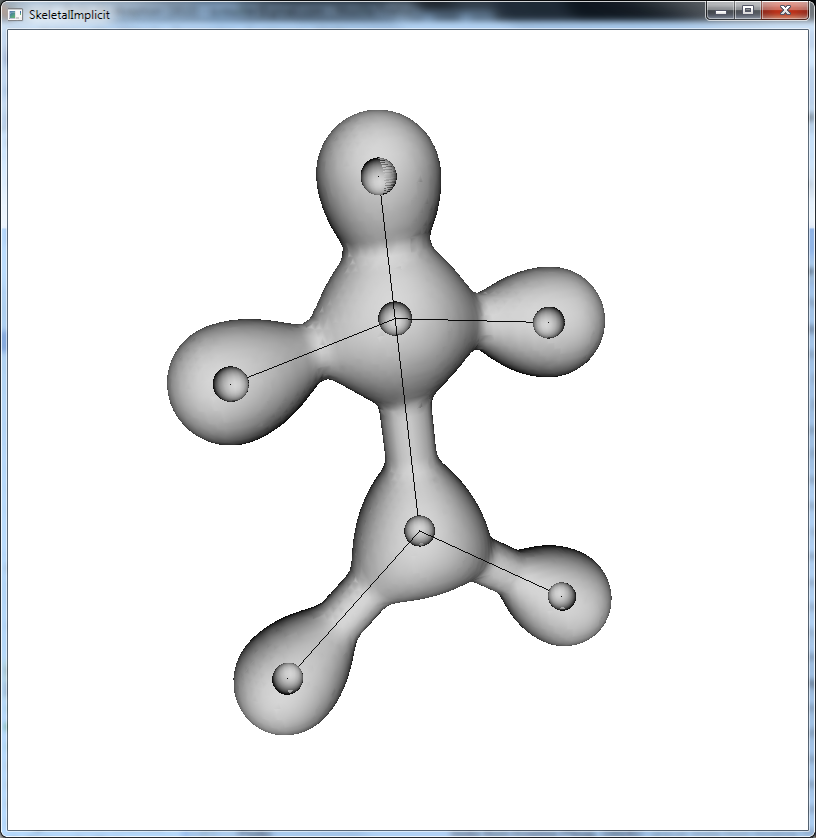
\includegraphics[scale=0.3]{../pictures/metaGuy.png}
\caption{Implicit Skeleton polygonized}
\label{bilb}
\end{figure}

\begin{figure}[!h!]
\centering
\includegraphics[scale=0.3]{../pictures/metaskeleton.png}
\caption{Implicit Skeleton polygonized}
\label{bilb}
\end{figure}

\item{Brute force ray tracing}
I rendered a cube and ray-traced on the fragment shader 2 metaballs and a metatube, naive raymarching and root finding.

\begin{figure}[!h!]
\centering
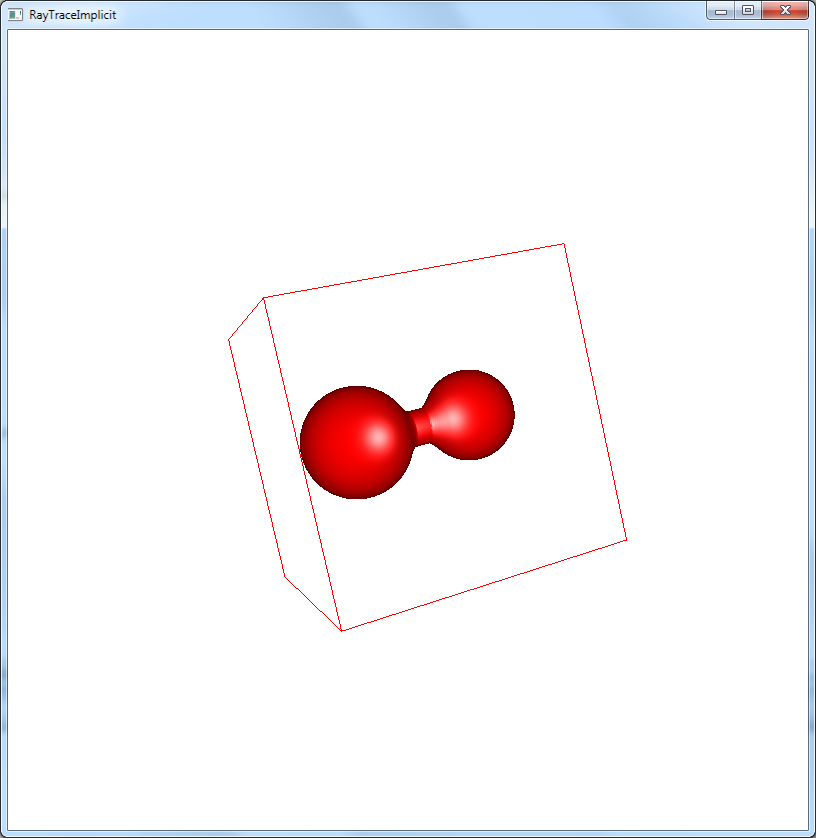
\includegraphics[scale=0.3]{../pictures/raytraceMetaballsandTube.png}
\caption{2 metaballs and a metatube raytraced on the GPU}
\label{bilb}
\end{figure}

\end{itemize}

\clearpage
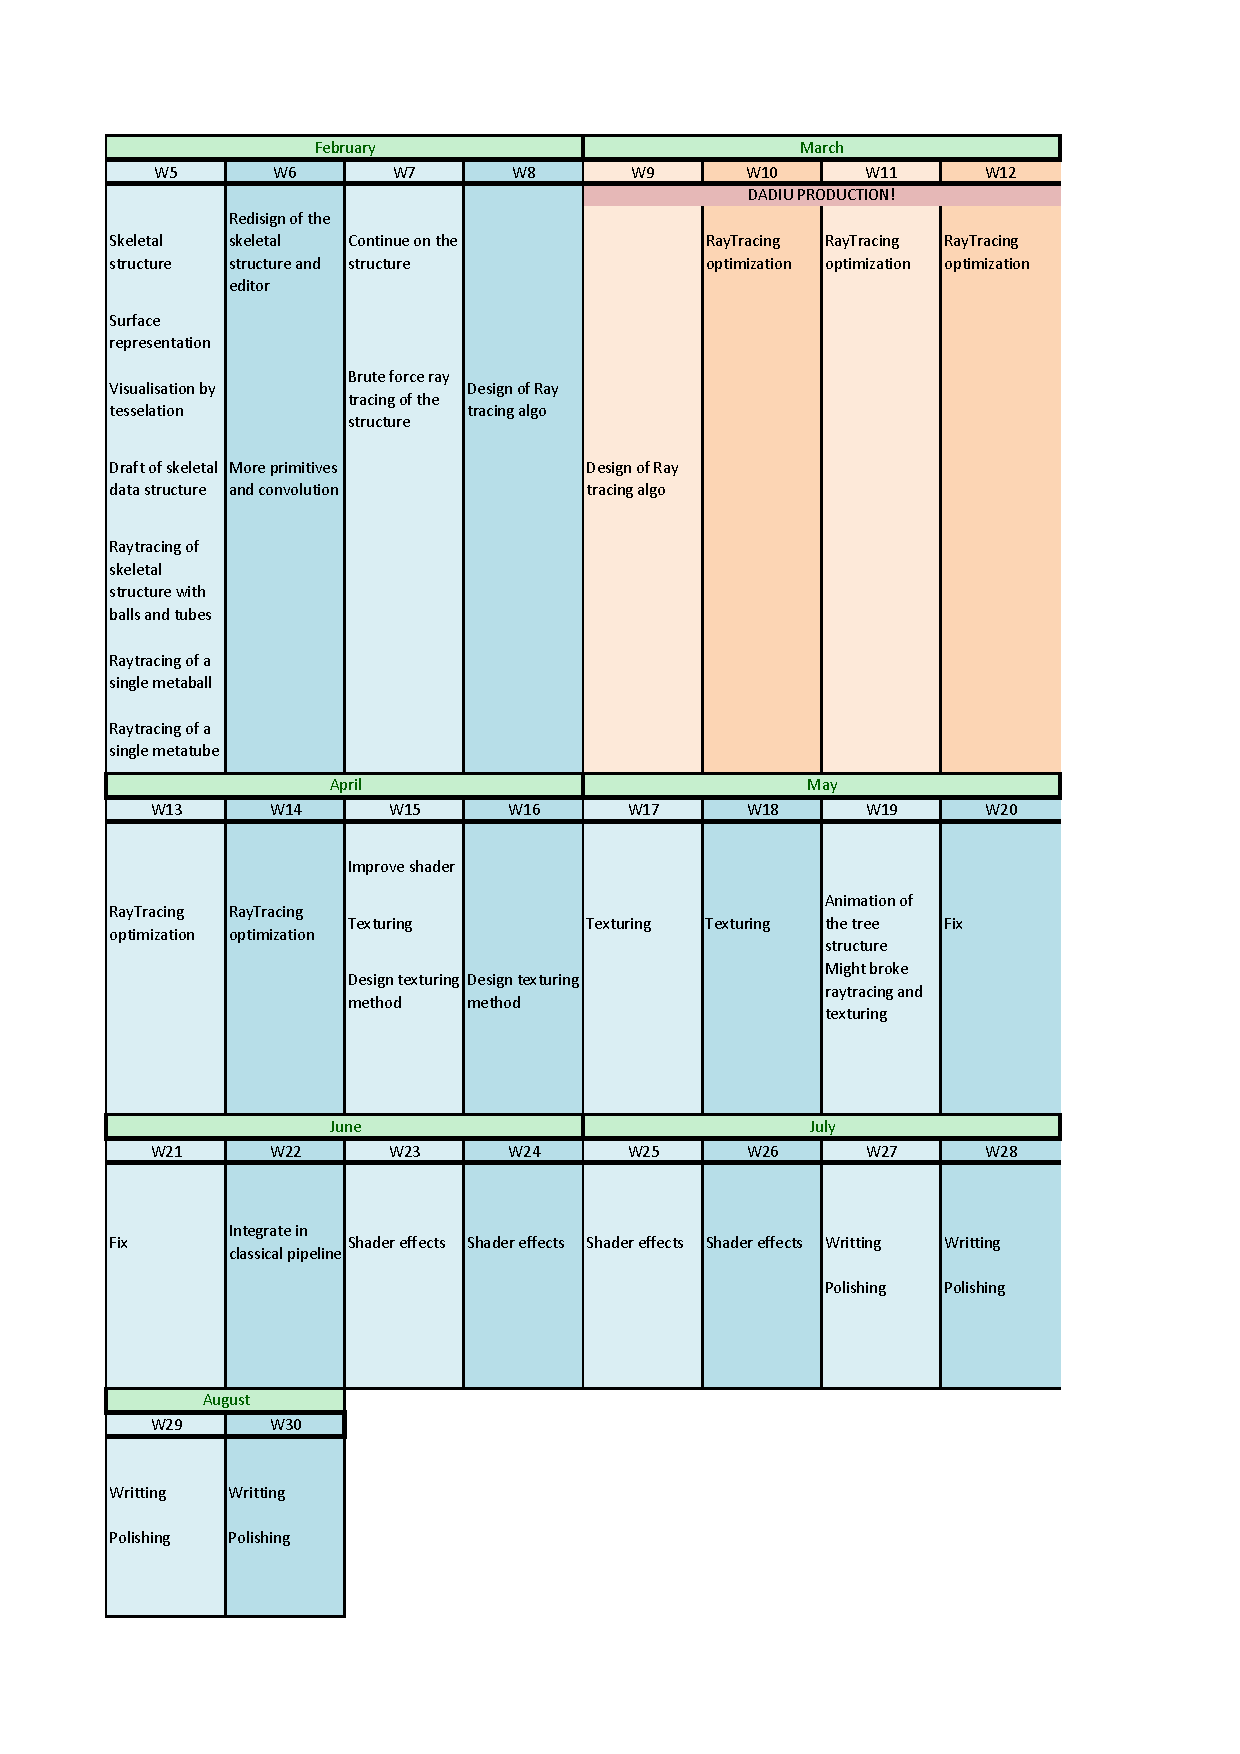
\includepdf{../../../projectPlan07-02.pdf} 

\bibliography{../../references} 
\bibliographystyle{alpha}

\end{document}
